\documentclass[a4paper,11pt,english]{article}
\usepackage{standalone}
\usepackage{tikz}
\usetikzlibrary{decorations.pathreplacing,arrows.meta,shapes}
\usepackage{tcolorbox}
\tcbuselibrary{breakable,skins}
\usepackage{babel}
\usepackage{booktabs}
\usepackage[colorlinks,pdfstartview=FitH,bookmarks,pdfcenterwindow]{hyperref}
\usepackage[capitalise]{cleveref}

\usepackage{protocol_version}

\definecolor{base03}{RGB}{000, 043, 054}
\definecolor{base02}{RGB}{007, 054, 066}
\definecolor{base01}{RGB}{088, 110, 117}
\definecolor{base00}{RGB}{101, 123, 131}
\definecolor{base0}{RGB}{131, 148, 150}
\definecolor{base1}{RGB}{147, 161, 161}
\definecolor{base2}{RGB}{238, 232, 213}
\definecolor{base3}{RGB}{253, 246, 227}
\definecolor{yellow}{RGB}{181, 137, 000}
\definecolor{orange}{RGB}{203, 075, 022}
\definecolor{red}{RGB}{220, 050, 047}
\definecolor{magenta}{RGB}{211, 054, 130}
\definecolor{violet}{RGB}{108, 113, 196}
\definecolor{blue}{RGB}{038, 139, 210}
\definecolor{cyan}{RGB}{042, 161, 152}
\definecolor{green}{RGB}{133, 153, 000}

\makeatletter

\def\@autolabel#1{%
\expandafter\let\csname old#1\expandafter\endcsname\csname#1\endcsname
\expandafter\def\csname @#1@label\endcsname[##1]##2{\csname old#1\endcsname{##2}\label{#1:##1}}
\expandafter\def\csname #1\endcsname{\expandafter\@ifnextchar[{\csname @#1@label\endcsname}{\csname old#1\endcsname}}
}

\@autolabel{part}
\@autolabel{section}
\@autolabel{subsection}
\@autolabel{subsubsection}
\@autolabel{paragraph}
\@autolabel{subparagraph}

\makeatother

\newtcolorbox{admobox}[3][]{
  breakable, skin=enhancedmiddle,
  boxrule=0mm, leftrule=2mm,
  colframe=#3, colback=#3!10, coltext=#3!30!black,
  title={#2}, attach title to upper, after title={.\ },
  fonttitle={\bfseries}, coltitle=black,
  #1
}
\def\notebox#1#2{
  \begin{admobox}{#1}{blue}
  #2
  \end{admobox}
}
\def\warnbox#1#2{
  \begin{admobox}{#1}{yellow}
  #2
  \end{admobox}
}
\def\errorbox#1#2{
  \begin{admobox}{#1}{red}
  #2
  \end{admobox}
}
\def\tipbox#1#2{
  \begin{admobox}{#1}{green}
  #2
  \end{admobox}
}

\def\fieldsize#1{
  \tikz[baseline=-.5ex]{
    \tikzset{fieldsize/.style={
      rectangle split,
      rectangle split parts=2,
      rectangle split horizontal,
      rectangle split part fill={violet,violet!10},
      rectangle split draw splits=false,
      rounded corners=2pt,
      rectangle split part align=base,
      draw=violet,
    }}
    \node[fieldsize] (var) {\textsc{\color{white}Size}\nodepart[text=violet!50!black]{two}#1};
  }
}

\title{OrbiPacket Protocol Specification - v\version}
\author{The OrbiSat Oeiras Team}
\date{}

\begin{document}
\maketitle
\documentclass{standalone}
\usepackage{tikz}
\usetikzlibrary{decorations.pathreplacing,arrows.meta}


\begin{document}
\definecolor{base03}{RGB}{000, 043, 054}%
\definecolor{base02}{RGB}{007, 054, 066}%
\definecolor{base01}{RGB}{088, 110, 117}%
\definecolor{base00}{RGB}{101, 123, 131}%
\definecolor{base0}{RGB}{131, 148, 150}%
\definecolor{base1}{RGB}{147, 161, 161}%
\definecolor{base2}{RGB}{238, 232, 213}%
\definecolor{base3}{RGB}{253, 246, 227}%
\definecolor{yellow}{RGB}{181, 137, 000}%
\definecolor{orange}{RGB}{203, 075, 022}%
\definecolor{red}{RGB}{220, 050, 047}%
\definecolor{magenta}{RGB}{211, 054, 130}%
\definecolor{violet}{RGB}{108, 113, 196}%
\definecolor{blue}{RGB}{038, 139, 210}%
\definecolor{cyan}{RGB}{042, 161, 152}%
\definecolor{green}{RGB}{133, 153, 000}%
\def\field[#1](#2)(#3)#4{\fill[#1,draw=base03] (#2) rectangle ++(#3) node[midway,text=base3,align=center] {#4};}%
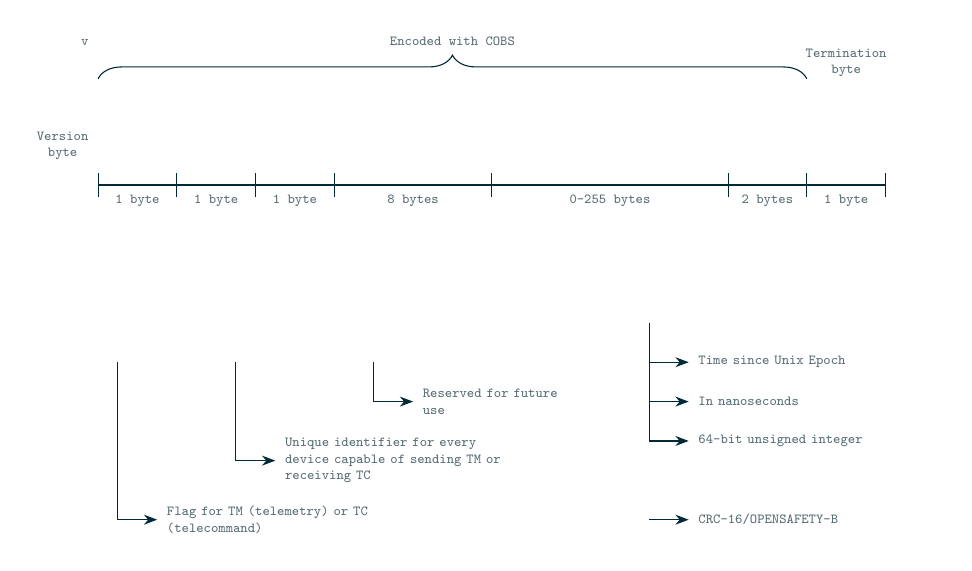
\begin{tikzpicture}[yscale=-1,draw=base03,every node/.style={font=\tiny\ttfamily,text=base01}]
    \node[above left] at (0,-.4) {v\version};
    % Full packet
    \field[blue](0,0)(5,.5){HEADER}
    \field[base02](0,.5)(1,.5){0x\versionbyte}
    \field[violet](1,.5)(1,.5){LENGTH}
    \field[magenta](2,.5)(1,.5){CONTROL}
    \field[cyan](3,.5)(2,.5){TIMESTAMP}
    \field[base00](5,0)(3,1){PAYLOAD}
    \field[green](8,0)(1,1){CRC}
    \field[base02](9,0)(1,1){0x00}
    % Field sizes
    \draw (0,1.25) -- ++(10,0);
    \foreach\x in {0,1,2,3,5,8,9,10}{
            \draw (\x,1.1) -- ++(0,.3);
        }
    \node[below] at (.5,1.25) {1 byte};
    \node[below] at (1.5,1.25) {1 byte};
    \node[below] at (2.5,1.25) {1 byte};
    \node[below] at (4,1.25) {8 bytes};
    \node[below] at (6.5,1.25) {0-255 bytes};
    \node[below] at (8.5,1.25) {2 bytes};
    \node[below] at (9.5,1.25) {1 byte};
    % Annotations
    \node[left,align=center] at (0,.75) {Version\\byte};
    \node[above,align=center] at (9.5,0) {Termination\\byte};
    \draw[decorate,decoration={brace,amplitude=.3cm}] (0,-.1) -- ++(9,0) node [midway,above=.3cm] {Encoded with COBS};
    % Control byte
    \field[magenta](0,2.5)(4,.5){CONTROL}
    \field[yellow](0,3)(.5,.5){TM/\\TC}
    \field[orange](.5,3)(2.5,.5){DEVICE ID}
    \field[red](3,3)(1,.5){RESERVED}
    \draw[-Stealth] (3.5,3.5) |- ++(.5,.5) node[right,align=left,text width=2cm] {Reserved for future use};
    \draw[-Stealth] (1.75,3.5) |- ++(.5,1.25) node[right,align=left,text width=3cm] {Unique identifier for every device capable of sending TM or receiving TC};
    \draw[-Stealth] (.25,3.5) |- ++(.5,2) node[right,align=left,text width=3cm] {Flag for TM (telemetry) or TC (telecommand)};
    % Timestamp
    \field[cyan](6,2.5)(2,.5){TIMESTAMP}
    \draw[-Stealth] (7,3) |- ++(.5,.5) node[right,align=left,text width=3cm] {Time since Unix Epoch};
    \draw[-Stealth] (7,3) |- ++(.5,1) node[right,align=left,text width=3cm] {In nanoseconds};
    \draw[-Stealth] (7,3) |- ++(.5,1.5) node[right,align=left,text width=3cm] {64-bit unsigned integer};
    % Crc
    \field[green](6,5)(1,1){CRC}
    \draw[-Stealth] (7,5.5) -- ++(.5,0) node[right,align=left]{CRC-16/OPENSAFETY-B};
\end{tikzpicture}
\end{document}
\tableofcontents

\section{Introduction}

OrbiPacket is a packet-based communication protocol. It was created specifically for communication with CanSat devices. These devices can be fitted with very diverse electronics, and are often resource-constrained. Thus, this protocol has the goals of being simple and easy to use while providing decent efficiency and minimal overhead.

\notebox{A bit of history}{
  The OrbiSat Oeiras team first participated in the CanSat Portugal competition in 2023/2024, being one of the finalists of the 11th edition. Several issues on all fronts meant no data was received during the CanSat's descent. The next year, wanting to get everything right, the team's firmware developer (aka me, Levi Gomes) decided sending data over text wasn't neither efficient nor rigorous enough. So, after some effort, the first version of OrbiPacket was born during the 12th edition of the competition, in 2024/2025. And in case you're curious... no, we still didn't get any data.
}

\section{Packet Structure}

Each packet consists of the following fields, which must be encoded in the specified order:

\begin{table}[h]
  \centering
  \begin{tabular}{ll}
    \toprule
    Field                     & Size (bytes) \\
    \midrule
    \textbf{Header}           & 11           \\
    Version                   & 1            \\
    Length                    & 1            \\
    Control                   & 1            \\
    Timestamp                 & 8            \\
    \textbf{Payload}          & 0-255        \\
    \textbf{CRC}              & 2            \\
    \textbf{Termination Byte} & 1            \\
    \bottomrule
  \end{tabular}
  \caption{Packet structure overview}
  \label{table:struct}
\end{table}

\subsection{Header}

\subsubsection{Version}
\fieldsize{1 byte}\\[8pt]
Indicates the protocol version. Breaking updates to the protocol increment this field to ensure backwards compatibility. The current version of the protocol (\version) specifies \texttt{0x\versionbyte} as the version byte.


\subsubsection{Length}
\fieldsize{1 byte}\\[8pt]
Specifies the size of the payload in bytes, ranging from 0 to 255.


\subsubsection{Control}
\fieldsize{1 byte}\\[8pt]
Encodes metadata about the packet type and device identifier. The following fields are specified from the highest bit to the lowest bit.
\begin{itemize}
  \item \textbf{TM/TC Flag}: 1 bit, where \texttt{0} indicates telemetry and \texttt{1} indicates a telecommand.
  \item \textbf{Device ID}: 5 bits, uniquely identifying the source device for TM or target device for TC. Note that device IDs should remain consistent across TM and TC packets.
  \item \textbf{Reserved Bits}: 2 bits, reserved for future use. The value of this field should be ignored.
\end{itemize}


\subsubsection{Timestamp}
\fieldsize{8 bytes}\\[8pt]
Represents the time since the Unix epoch in nanoseconds as a 64-bit unsigned integer.


\subsection{Payload}
\fieldsize{0–255 bytes}\\[8pt]
Contains application-specific data, such as telemetry readings or command instructions. The structure of the payload is currently up to the application, but that may be subject to change in future versions.


\subsection{CRC}
\fieldsize{2 bytes}\\[8pt]
Cyclic redundancy check value computed over all preceding fields (excluding the termination byte). The generator polynomial used by the protocol is \href{https://reveng.sourceforge.io/crc-catalogue/all.htm#crc.cat.crc-16-opensafety-b}{CRC-16/OPENSAFETY-B}, or \texttt{0xbaad} in Koopman's notation.


\subsection{Termination Byte}
\fieldsize{1 byte}\\[8pt]
Marks the end of the packet, ensuring clear packet delimitation. Fixed at \texttt{0x00}.


\section{Field Order and Endianness}

Packet fields must be encoded in the specified order, as a byte string. Multi-byte fields are encoded in \textbf{little-endian}.

\section{Encoding}

To prevent the occurrence of the termination byte (\texttt{0x00}) within the packet, the protocol employs \textbf{COBS (Consistent Overhead Byte Stuffing)} encoding. This encoding is applied to all fields except the termination byte itself, simplifying parsing and improving error resilience.

\section{Packet Operations}

\subsection{Creation}
\begin{itemize}
  \item Packet fields, excluding the CRC and termination bytes, are converted into binary and chained together in the specified order.
  \item A CRC is computed over the resulting binary string, and appended to it.
  \item COBS encoding is applied to the entire binary string, and the termination byte is appended to it, concluding packet creation.
\end{itemize}

\subsection{Transmission}
\begin{itemize}
  \item Packets are transmitted in binary, over an application-specific digital or physical medium (e.g. radio).
\end{itemize}

\subsection{Reception}
\begin{itemize}
  \item Packets are decoded using COBS
  \item The packet structure is recovered from the decoded binary string.
\end{itemize}

\subsection{Validation}
\begin{itemize}
  \item Packets which don't start at \texttt{0x00} (the termination byte of the previous packet) are discarded. This allows for re-synchronization in case of a broken or lossy connection.
  \item Packets which cannot be properly decoded with COBS are discarded.
  \item Packets which fail CRC validation are discarded.
  \item Packets with erroneous length fields are discarded.
\end{itemize}

\subsection{Acknowledgment and Retransmission}
Acknowledgment of packets, and their retransmission in case of packet loss, is not currently required by the protocol. It is up to implementations to decide if, and how, this is handled.

\subsection{Version Negotiation}
No version negotiation strategy is enforced by the packed in the event of communicators having mismatched versions.


\section{Example Packet}

\begin{table}[h]
  \centering
  \begin{tabular}{lll}
    \toprule
    Field                & Example Value                       & Notes                     \\
    \midrule
    \textbf{Version}     & \texttt{0x\versionbyte}             & Protocol version \version \\
    \textbf{Length}      & \texttt{0x04}                       & Payload size: 4 bytes     \\
    \textbf{Control}     & \texttt{0x81}                       & Telecommand, Device ID 1  \\
    \textbf{Timestamp}   & \texttt{0x000001787ABCEF0123456789} & Example timestamp         \\
    \textbf{Payload}     & \texttt{0xDEADBEEF}                 & Application-specific data \\
    \textbf{CRC}         & \texttt{0x5A}                       & Example CRC value         \\
    \textbf{Termination} & \texttt{0x00}                       & Packet terminator         \\
    \bottomrule
  \end{tabular}
  \caption{An example packet}
  \label{table:example}
\end{table}

\section{Packet Overhead}

The fixed fields (header and CRC) result in a total, unencoded overhead of 13 bytes, so packet sizes range from 13 to 268 bytes, depending on payload length. COBS encoding has a maximum overhead of 1 byte per 254 bytes of unencoded data. Thus, accounting for the termination byte, the maximum overhead is 15 or 16 bytes per packet.

\section{Implementation Guidelines}

If available, use a reference implementation of the protocol for the chosen language. Otherwise, make sure to conform to the specifications of this document.

\subsection{Versioning}

The protocol is versioned using \href{https://semver.org/}{Semantic Versioning}. Breaking changes always increment the version byte. Implementations of the protocol must clearly specify to the end user the supported protocol versions.

\subsection{CRC Computation}

The generator polynomial used by the protocol is \href{https://reveng.sourceforge.io/crc-catalogue/all.htm#crc.cat.crc-16-opensafety-b}{CRC-16/OPENSAFETY-B}, or \texttt{0xbaad} in Koopman's notation. The maximum packet length (excluding the CRC and termination bytes) is 255 + 11 = 266 bytes or 2128 bits. According to \href{https://users.ece.cmu.edu/~koopman/crc/c16/0xbaad_len.txt}{Koopman's research}, this polynomial can protect 7985 bits at a Hamming distance of 4 and 108 bits (equivalent to 2 bytes of payload data) at a Hamming distance of 5, with negligible protected lengths for higher Hamming distances. This is deemed sufficient for this protocol. The parameters of this polynomial are:

\begin{itemize}
  \item \textit{width}: \texttt{16}
  \item \textit{poly}: \texttt{0x755b}
  \item \textit{init}: \texttt{0x0000}
  \item \textit{refin}: \texttt{false}
  \item \textit{refout}: \texttt{false}
  \item \textit{xorout}: \texttt{0x0000}
  \item \textit{check}: \texttt{0x20fe}
  \item \textit{residue}: \texttt{0x0000}
\end{itemize}

\subsection{COBS}
Reference implementations of the COBS algorithm should be used whenever possible. Otherwise, refer to the literature for details on the encoding and decoding process. The packet data should be stuffed to remove the termination byte, that is, \texttt{0x00}.

\end{document}